
\subsection{Answers}
\begin{table}[htb]%
\begin{center}%
\caption{Q18: Which MPI thread support are you using?}%
\label{tab:Q18-ans}%
\begin{tabular}{l|l|r}%
\hline%
Choice & Abbrv. & \# Answers \\%
\hline%
MPI\_THREAD\_SINGLE & SINGLE & 238 (28.7\%) \\%
MPI\_THREAD\_FUNNELED & FUNNELED & 145 (17.5\%) \\%
MPI\_THREAD\_SERIALIZED & SERIALIZED & 99 (11.9\%) \\%
MPI\_THREAD\_MULTIPLE & MULTIPLE & 261 (31.4\%) \\%
I have never called MPI\_INIT\_THREAD & never used & 267 (32.2\%) \\%
I do not know or I do not care. & do not know/care & 168 (20.2\%) \\%
\hline%
\multicolumn{2}{c}{total} & 1178 (830)\\%
\hline%
\end{tabular}%
\end{center}%
\end{table}%


\begin{figure}[htb]
\begin{center}
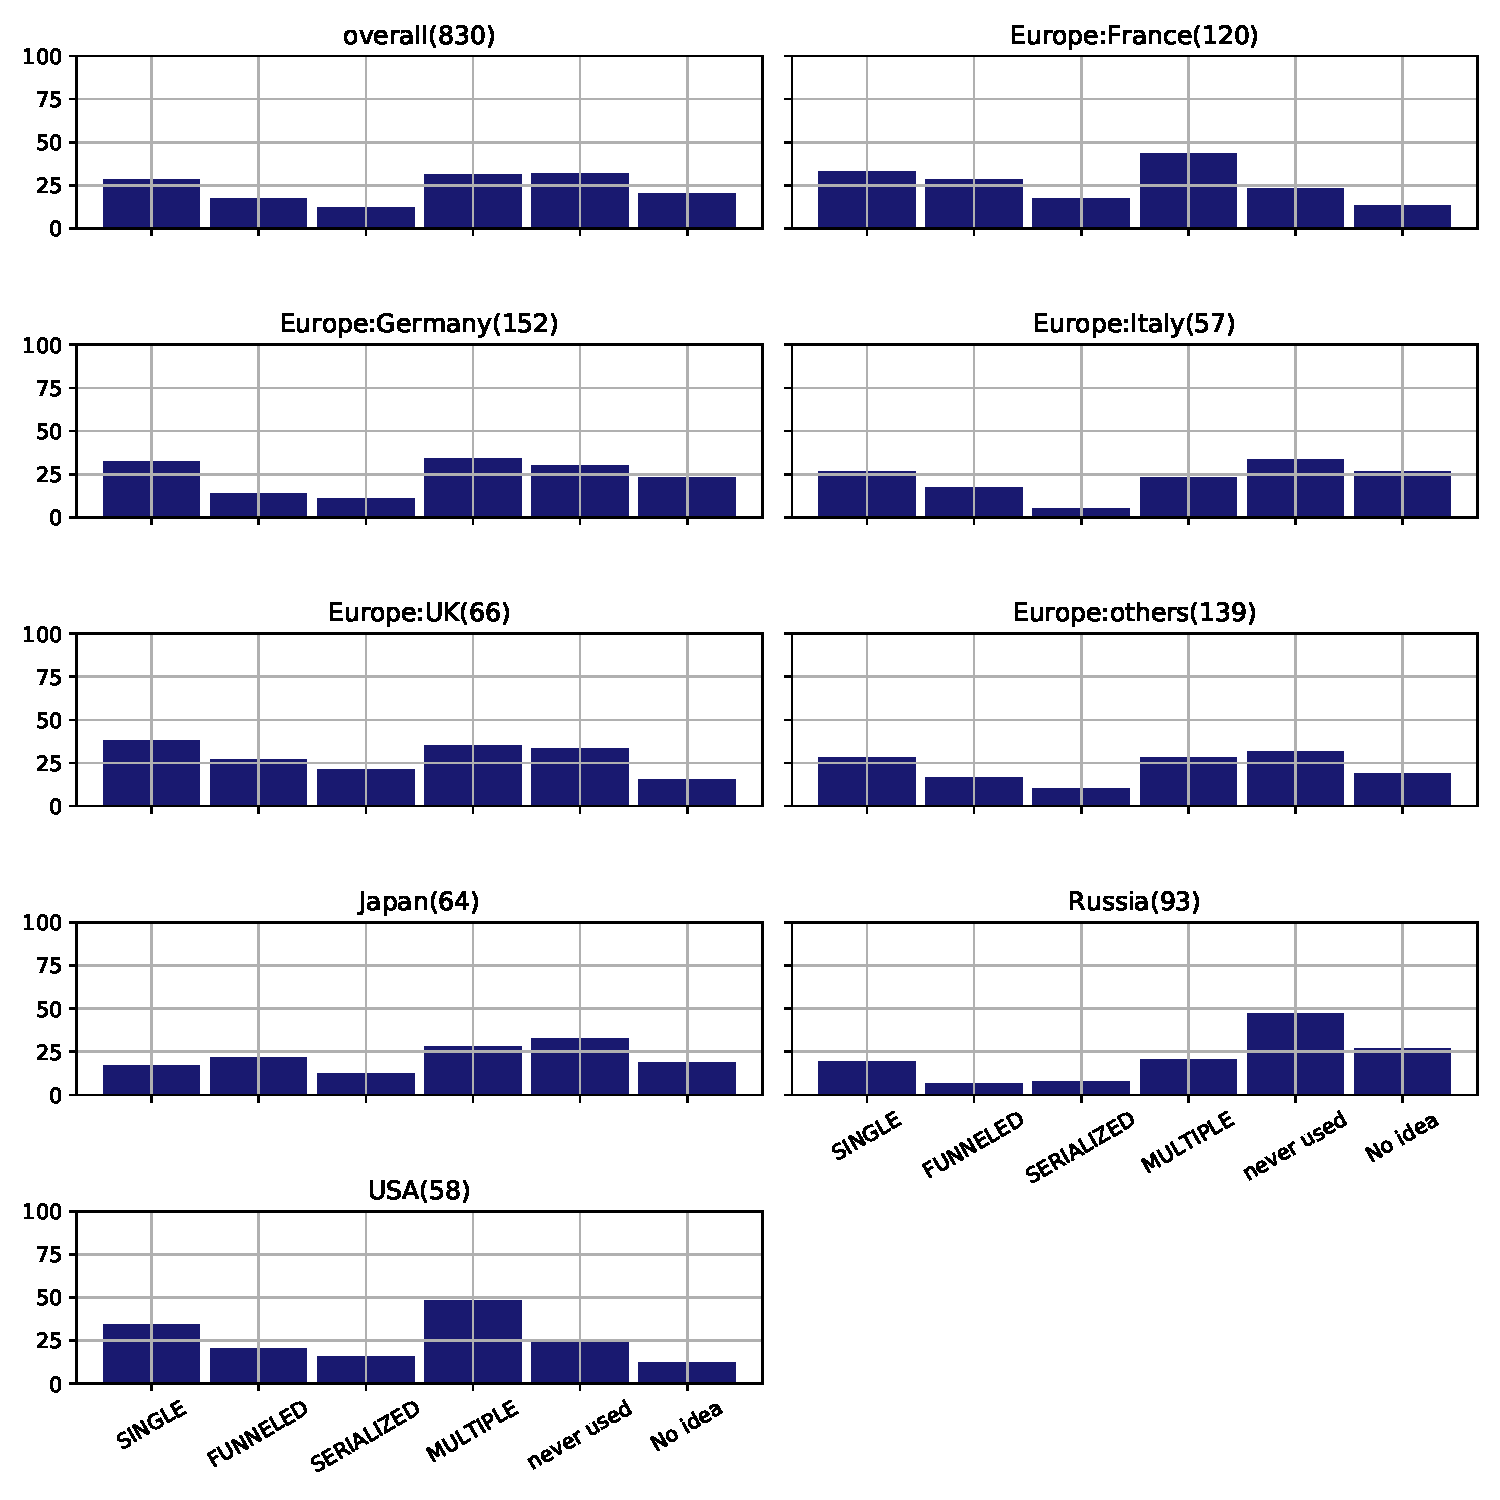
\includegraphics[width=10cm]{../pdfs/Q18.pdf}
\caption{Simple analysis: Q18}
\label{fig:Q18}
\end{center}
\end{figure}

The support of multi-threading in MPI is done in different ways (MPI\_THREAD\_SINGLE
MPI\_THREAD\_FUNNELED, MPI\_THREAD\_SERIALIZED, MPI\_THREAD\_MULTIPLE, in order of
decreasing semantic restriction). If used the most used option (42\%) are either
MPI\_THREAD\_SINGLE or MPI\_THREAD\_MULTIPLE which are the at the two and of the
spectrum in terms of thread support: most users either want a full support or a
limited support. Moreover, almost 40\% of the respondent have no usage of thread
support in their program. Region-wise, we see that in the USA, thread support is more used
than in other region and the most used option is MPI\_THREAD\_MULTIPLE which is
the least restrictive option. 

